\documentclass{beamer}
\usepackage{amsmath}
\usepackage{graphicx}
%Information to be included in the title page:
\title{Induction-induction}
\author{Thomas Postuma, Pieter-Jan Lavaerts}
\institute{Radboud University}
\date{2024}

\begin{document}

\frame{\titlepage}

\begin{frame}
    \frametitle{Inductive-Inductive buildings}
	{\footnotesize
	\begin{align*}
		\text{ground} &: \text{Platform},\\
		\text{extension} &: ((p : \text{Platform}) \times \text{Building}(p)) \rightarrow \text{Platform} ,\\
		\text{onTop} &: (p : \text{Platform}) \rightarrow \text{Building}(p) ,\\
		\text{hangingUnder} &: ((p : \text{Platform}) \times (b : \text{Building}(p))) \rightarrow \text{Building}(\text{extension}(\langle p, b \rangle))
	\end{align*}
	}%
	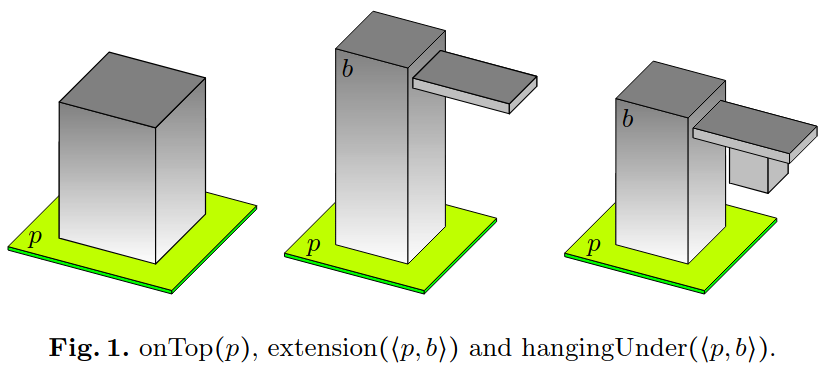
\includegraphics[width=\textwidth]{buildings}
\end{frame}

\begin{frame}
    \frametitle{Inductive-Inductive buildings (sigma notation)}
	{\footnotesize
	\begin{align*}
		\text{ground} &: \text{Platform},\\
		\text{extension} &: (\Sigma(p : \text{Platform}) \text{Building}(p)) \rightarrow \text{Platform} ,\\
		\text{onTop} &: (p : \text{Platform}) \rightarrow \text{Building}(p) ,\\
		\text{hangingUnder} &: (\Sigma(p : \text{Platform}) (b : \text{Building}(p))) \rightarrow \text{Building}(\text{extension}(\langle p, b \rangle))
	\end{align*}
	}%
	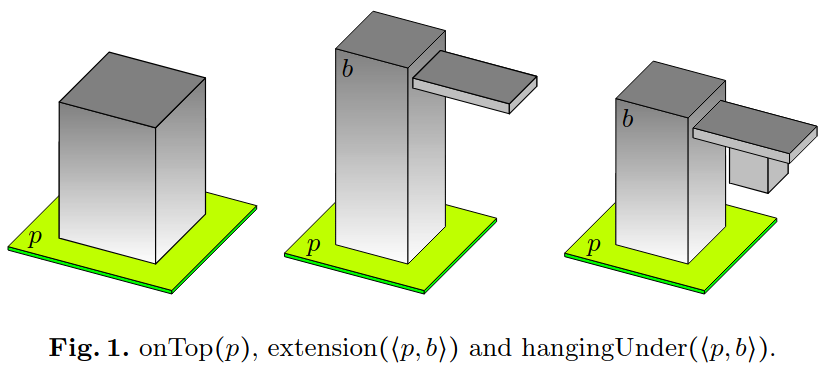
\includegraphics[width=\textwidth]{buildings}
\end{frame}

\begin{frame}
	\frametitle{Simultaneous inductive to Inductive-Inductive}

	Simultaneous inductive

	$$ \text{intro}_A : \Phi_A(A, B) \rightarrow A \quad\quad \text{intro}_B : \Phi_B(A, B) \rightarrow B $$

	Inductive-inductive

	$$ \text{intro}_B : (a : \Phi_B(A, B)) \rightarrow B(i_{A,B} (a)) $$

\end{frame}

\begin{frame}
    \frametitle{Axiomatisation using coding}

	$$ SP_A \quad\quad SP_B $$

    For constructors for instance
     
	$$ \text{extension} : ((p : \text{Platform)} \times \text{Building}(p)) \rightarrow \text{Platform} $$

\end{frame}

\end{document}
